\section{数据集与任务设计}

\subsection{Figure 1：FORGE 的整体逻辑}

Figure~\ref{fig:forge-figure1} 是论文的总览图，可以从数据基础、细粒度语义、任务设计和评测/训练资源四个层面理解。

\begin{figure}[H]
    \centering
    
\includegraphics[width=0.96\textwidth]{figures/figure1.png}
    \caption{FORGE 的整体流程、与旧 benchmark 的差异，以及不同模型在各任务上的总体表现。}
    \label{fig:forge-figure1}
\end{figure}

第一层是 multimodal data foundation。FORGE 同时包含真实世界 2D 图像和 3D 点云。制造任务往往不能只靠单张 RGB 图像完成，因为零件长度、厚度、螺纹、表面凹陷、缺口和装配关系都与几何结构密切相关。

第二层是 fine-grained semantic annotations。FORGE 不只标注“这是螺丝/螺母”，而是进一步标到型号、规格、兼容关系和缺陷类型。例如 M10 与 M20 都可能属于同一类工件，但在装配中不能互换。这样的标注使 benchmark 真正进入制造语义层面。

第三层是三类任务：Workpiece Verification、Structural Surface Inspection 和 Assembly Verification。它们分别对应制造中的分拣/混料检查、表面质检和装配检查。

第四层是 baseline evaluations 与 actionable training resource。论文不仅用 FORGE 测试当前 SOTA MLLM，还证明这些标注可以用于 SFT，使小模型在 held-out 场景中获得显著提升。

\subsection{Table 1：与已有 Benchmark 的区别}

Table~\ref{fig:forge-table1} 说明 FORGE 与已有制造/工业 benchmark 的区别。表格重点比较输入模态、数据来源、语义粒度、可用性和样本量。

\begin{figure}[H]
    \centering
    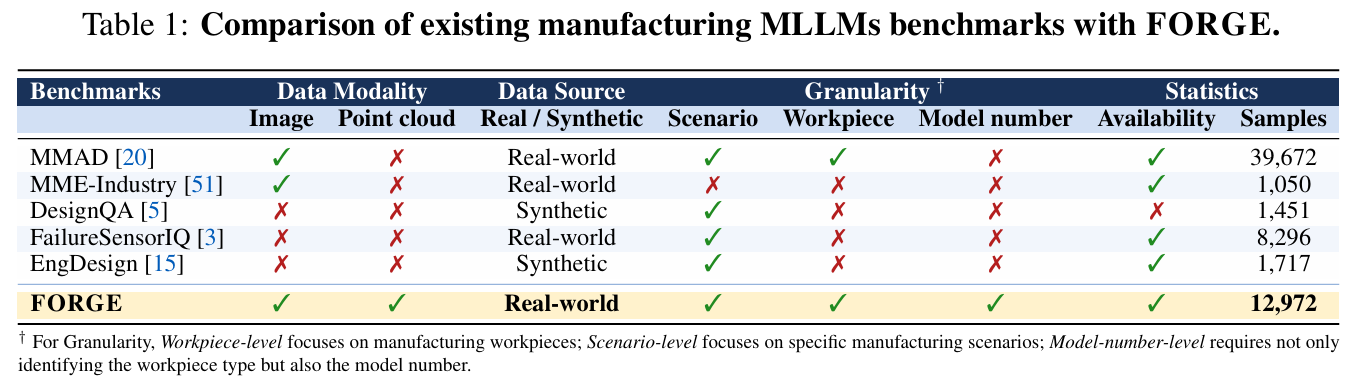
\includegraphics[width=0.96\textwidth]{figures/table1.png}
    \caption{FORGE 与已有制造业多模态 benchmark 的对比。}
    \label{fig:forge-table1}
\end{figure}

FORGE 的关键不在于样本量最大，而在于覆盖维度最完整：真实数据、图像与点云、多粒度语义、型号级标注以及贴近制造现场的任务。已有数据集常见不足包括：只支持图像、不包含点云、依赖合成数据、粒度停留在场景级或工件级、缺少型号级语义，或任务更偏工程文档和故障诊断而不是生产现场工件理解。

表中的 granularity 尤其重要。scenario-level 关注场景层面，workpiece-level 关注工件类别，model-number-level 则要求识别具体型号。FORGE 的独特性就在于进入型号级语义：模型不仅要知道这是 nut，还要知道它是不是 M14，以及它是否与当前装配规格匹配。

\subsection{Figure 2：三类制造任务}

Figure~\ref{fig:forge-figure2} 展示了 FORGE 的三个具体任务。它不是抽象描述 benchmark，而是在说明模型输入是什么、问题如何提问、输出需要判断什么。

\begin{figure}[H]
    \centering
    
\includegraphics[width=0.96\textwidth]{figures/figure2.png}
    \caption{FORGE 的三类任务：工件验证、结构表面检测和装配验证。}
    \label{fig:forge-figure2}
\end{figure}

\subsection{Workpiece Verification}

工件验证任务模拟制造中的分拣或混料检测。给定一批工件，模型需要判断哪些工件不属于当前批次。错误可能有两类：一种是完全不同类别的工件，例如混入 wing screw；另一种是同类但型号不对，例如应为 M14 却混入 M16。

这个任务表面上像“找不同”，本质上考四层能力：识别单个工件、比较工件之间是否属于同一批、区分类别错误和型号错误、把结果映射到选项字母。型号差异通常比类别差异更细微，也更贴近真实制造风险。

\subsection{Structural Surface Inspection}

结构表面检测任务接近工业质检。模型需要先判断工件是否正常，再在异常时判断缺陷类型。论文涉及的典型缺陷包括 crack、cut、deformation、dent 和 good。

这一任务在实验中最难，因为它依赖微观形态分析。模型需要关注表面纹理、局部缺口、细小凹陷和形变，而不是只识别宏观工件类别。当前 MLLM 往往擅长宏观语义，但不擅长这类细粒度 morphology。

\subsection{Assembly Verification}

装配验证任务要求模型检查当前装配是否满足规格。错误可能来自型号不匹配、零件长度错误、多装零件、少装零件或装配关系不正确。

这项任务最偏推理。模型需要读懂装配规格，识别图中部件，完成计数和配对，再判断哪个部件多余、缺失或不兼容。它考的是零件识别、数量约束、装配兼容性和逻辑一致性，而不是单件分类。

\subsection{2D 图像、3D 点云与三视图策略}

FORGE 同时使用图像和点云。点云可写为

\begin{equation}
    P = \{(x_i,y_i,z_i)\}_{i=1}^{N},
\end{equation}

其中每个点表示物体表面采样位置。主流通用 MLLM 通常没有原生 3D 编码器，即没有专门处理点云、mesh 或 voxel 的模块。它们更擅长输入文本和图像，而不是直接处理三维坐标集合。

一种直觉做法是把点云坐标序列化成文本，例如

\begin{verbatim}
Point 1: (12, 35, 8)
Point 2: (13, 35, 9)
...
\end{verbatim}

但这种方式低效，因为空间邻域关系不自然，token 序列很长，语言模型也不擅长从数字串恢复三维形状。论文的瓶颈分析也显示，raw point cloud text input 的效果接近随机。

因此 FORGE 采用三视图（3V）投影策略：把同一个点云从 front、side、top 三个方向渲染为普通 2D 图像。单个视角会丢掉一维信息，但三个互补视角能保留工件轮廓、长度、厚度、局部结构和部分缺陷痕迹。更重要的是，三视图输出仍是标准图像，通用 MLLM 可以直接使用现有视觉编码器处理。

使用专门 3D 模型当然可能更适合点云，但那会偏离本文目标。FORGE 想评估的是通用 foundation MLLM 的制造认知能力，而不是专门 3D backbone 的几何建模能力。因此三视图是一种实用折中：既保留关键几何结构，又兼容标准 MLLM 输入接口。
